\label{chap:machine_model}
This chapter describes the machine model upon which the PDP operates to motivate current and future use-cases. Each component is discussed in detail with a focus on how these components map to the operations within traditional IRSPs. Finally, it provides an example of how utilizing compositing and PDP in tandem could provide performance benefits.

\section{Hardware Mapping}
    This section discusses the different processes of an IRSP system in order to show how these processes can be mapped to an abstract PDP architecture that could be implemented with different kinds of physical hardware. The purpose is to show the reader that with the PDP the traditional IRSP system can be scaled to a multitude of different parallel setups.

    Traditional IRSP systems are composed of four distinct processes: scene generation, non-uniformity correction (with data reordering), digital to analog conversion, and projection as indicated in Figure~\ref{fig:typical_projection} in Chapter~\ref{chap:background}. Scene generation and non-uniformity correction may or may not operate within the same hardware, but from an implementation perspective are segmented into a pipeline operation irrespective of the physical hardware as shown in Figure~\ref{fig:typical_projection_hardware}. Digital to analog conversion on the other hand is always performed with separate electronics that are located close to an array as indicated in Chapter~\ref{sec:close_support_electronics}.

    \begin{figure}
        \centering
        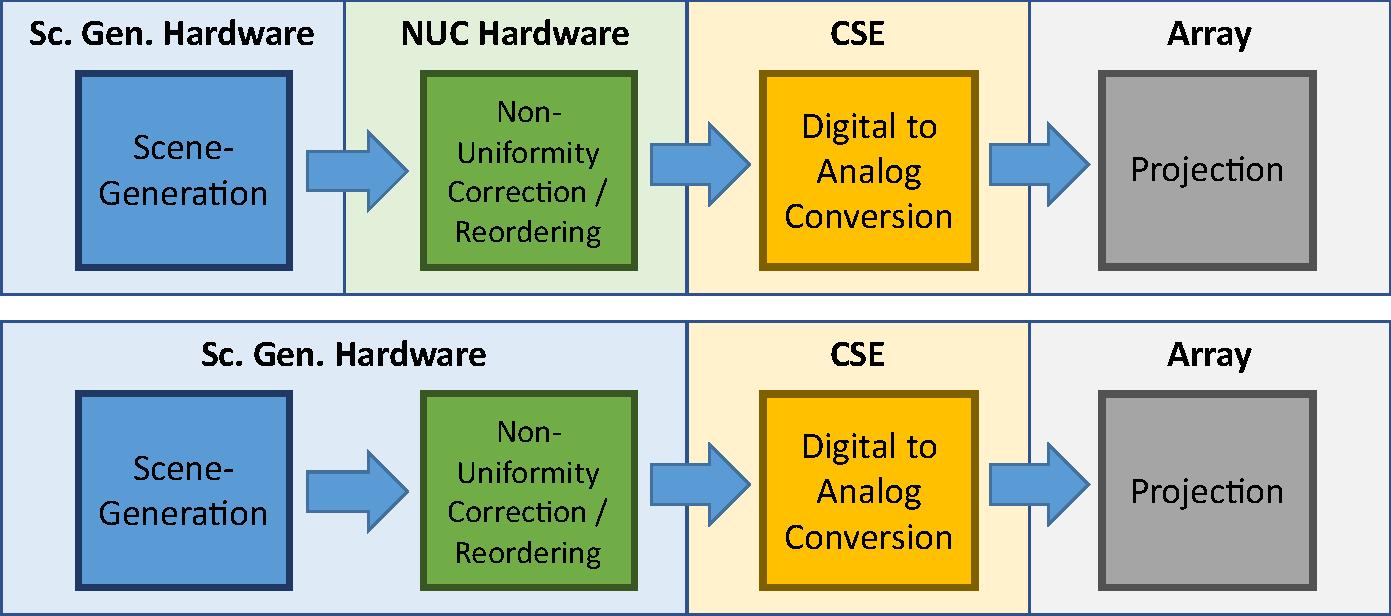
\includegraphics[width=1.0\textwidth]{fig/typical_projection_system_hardware.pdf}
        \caption{Hardware Mapping of an IRLED Projection Process}
        \label{fig:typical_projection_hardware}
    \end{figure}

    Given that these processes are separate, they can be mapped readily to a machine model which represents an abstraction of an IRSP system utilizing the PDP as shown in Figure~\ref{fig:amm}. The Abstract Machine Model (AMM) separates the system operation of an IRSP system into three main components scene generation, compositing, and display. Scene generation consist of image generation just as in traditional IRSPs; however, more than one scene generator can be utilized to generate partial imagery. Compositing is the process of combining partial images into full PDP frames as well as performing non-uniformity correction and data reordering. More than one compositor is allowed for the purposes of scaling. an IRLED Array tile represents both an array tile and its supporting electronics. Between the components exist abstract links which operate using the PDP. Compositor blocks and IRLED Array Tiles have a one-to-one relationship. The multiple CSE setup discussed in Chapter~\ref{sec:array_Interleaved_write_process} is an example of this type of setup. There is prior work on parallel scene generation and compositing specifically for hardware in the loop scene generation~\cite{CrowEtAl2006, ShyuEtAl2011, MorrisEtAl2011}.

    \begin{figure}
        \centering
        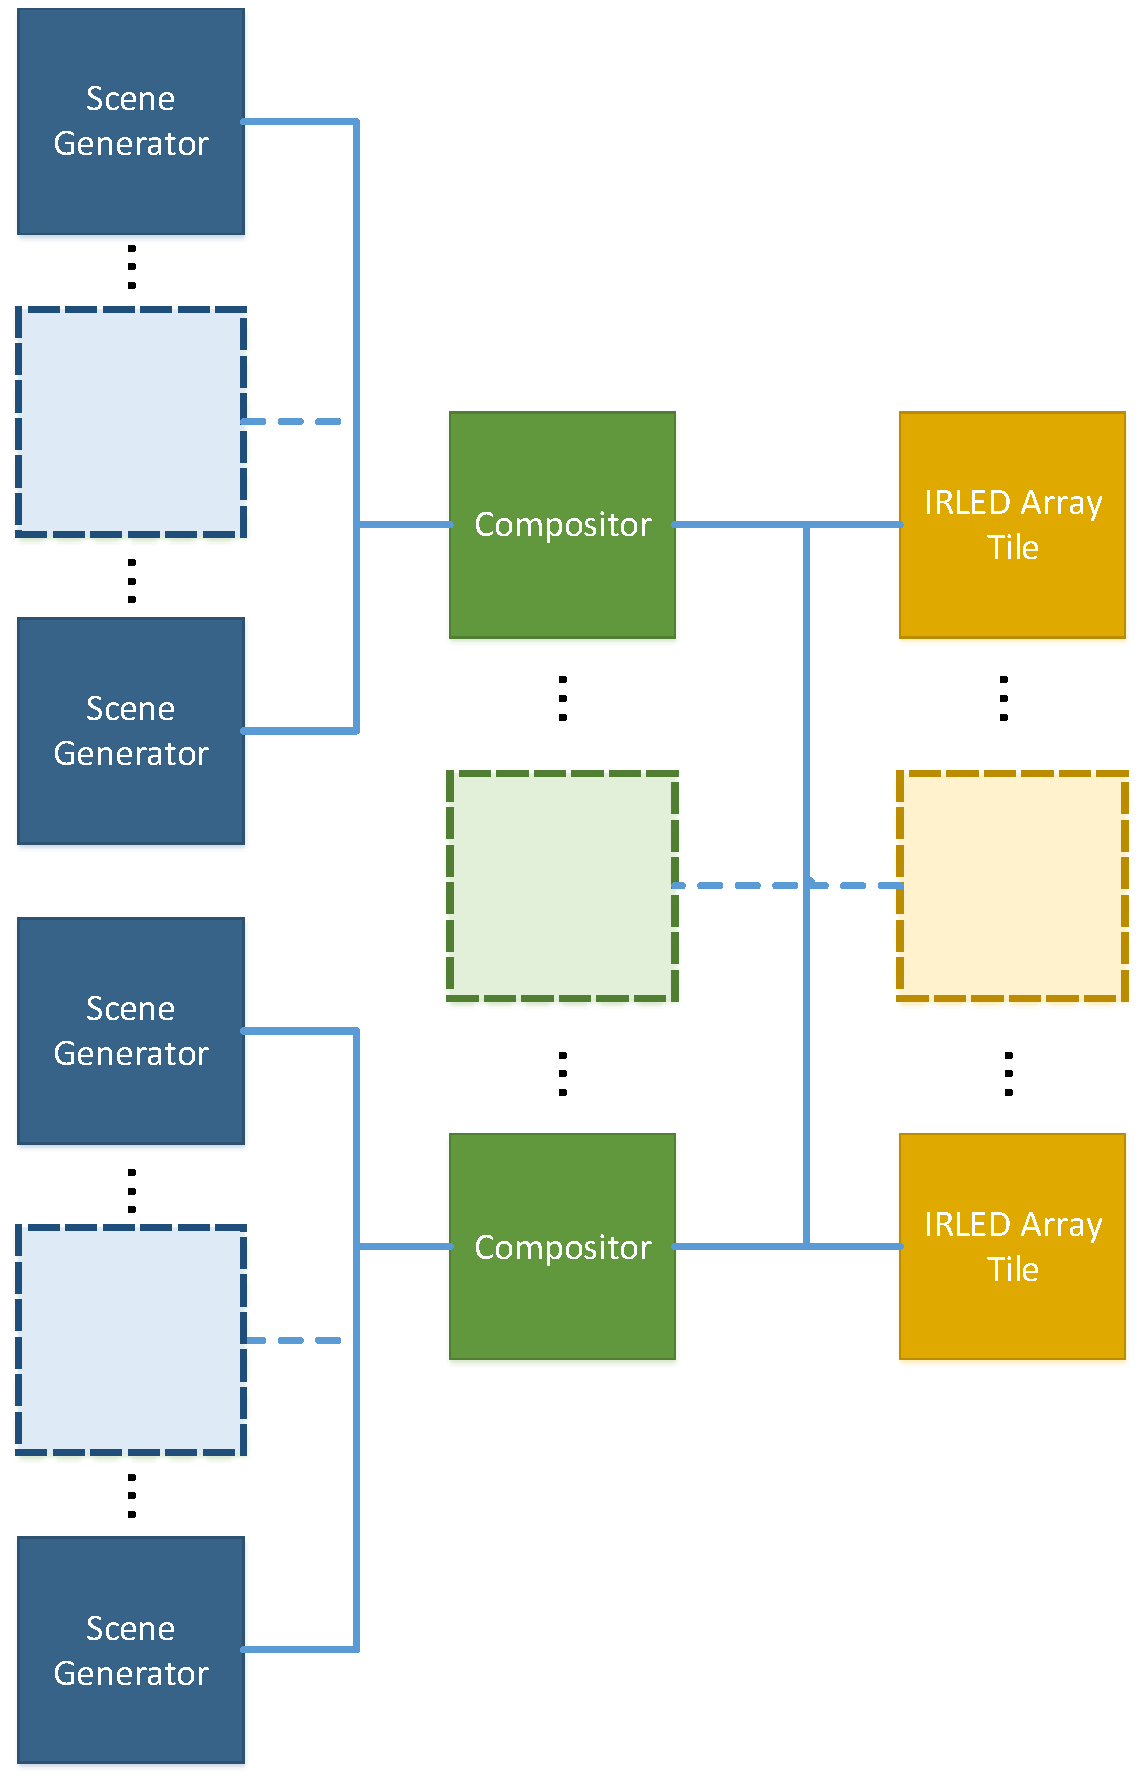
\includegraphics[width=0.83\textwidth]{fig/amm.pdf}
        \caption{Abstract Machine Model of the PDP architecture with 1-to-N relationships between components}
        \label{fig:amm}
    \end{figure}

    The relationship between these components remains abstracted in such a way that hardware components may be scaled to fit demand. At its most basic, a single scene generator, compositor, and IRLED array tile may be used just as in a traditional setup. For higher speed requirements, hardware components may be mapped as needed. As noted above, the links between components in the system utilize the PDP for communication, data-transfer, and synchronization. The compositing component differs from a traditional IRSP system in that it is responsible for taking imagery from many sources, possibly at different frame rates, and combining them into a single image for transmission to IRLED array tiles. This process is discussed in more detail in the following section.

\section{Compositing}
    \label{sec:compositing}
    This section discusses a compositing layer and analysis that could be implemented into a system utilizing the PDP. As noted previously, compositing is the process of combining two or more images into a single picture. In high-speed systems imagery could be generated in individual pieces and combined with a compositor layer. This process might be done by a single system or with separate systems.

    A general example of how compositing might look is shown in Figure~\ref{fig:compositing}. During the compositing process frame segments are ranked to determine which to send at high speeds, and which to send at low speeds for intelligent bandwidth utilization. Once segmented and ranked into non-overlapping speed classes, frame segments are transmitted at the necessary rate. Figure~\ref{fig:compositing_overlayed} shows the source segments overlayed with the image where one can see how each region maps to the image.

    \begin{figure}
        \centering
        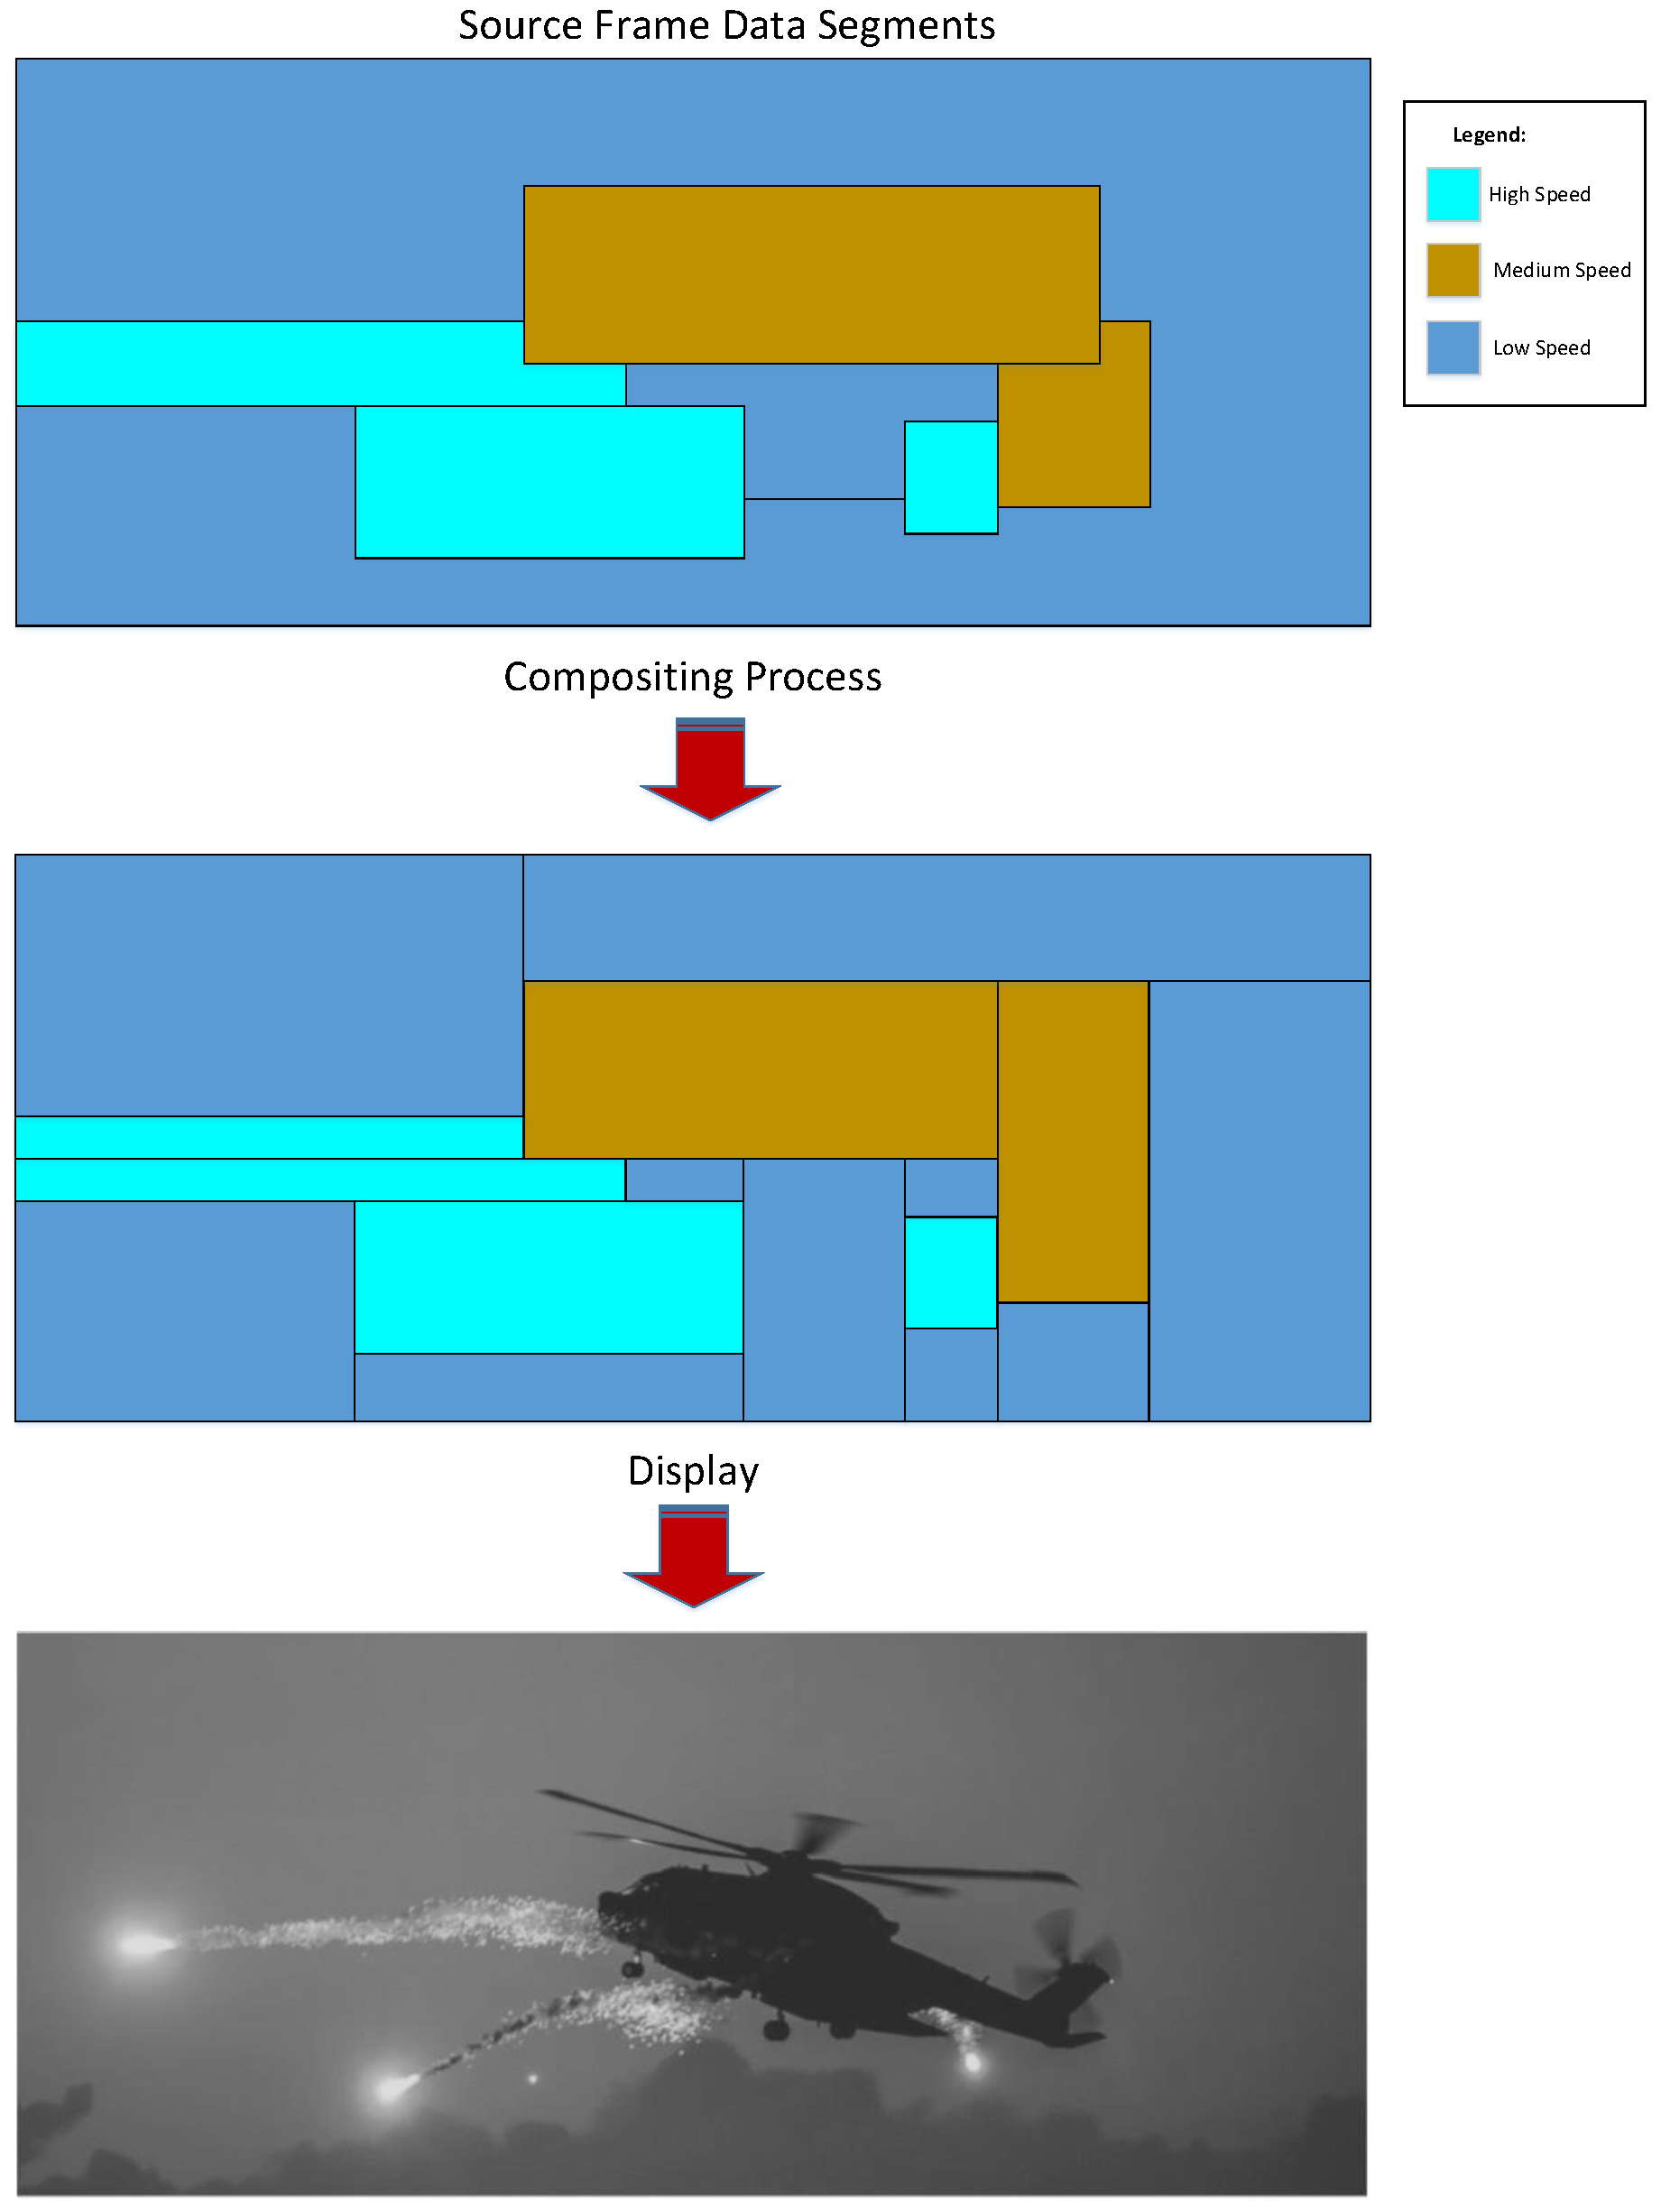
\includegraphics[width=1.0\textwidth]{fig/compositing.pdf}
        \caption{Compositing Process Example}
        \label{fig:compositing}
    \end{figure}

    \begin{figure}
        \centering
        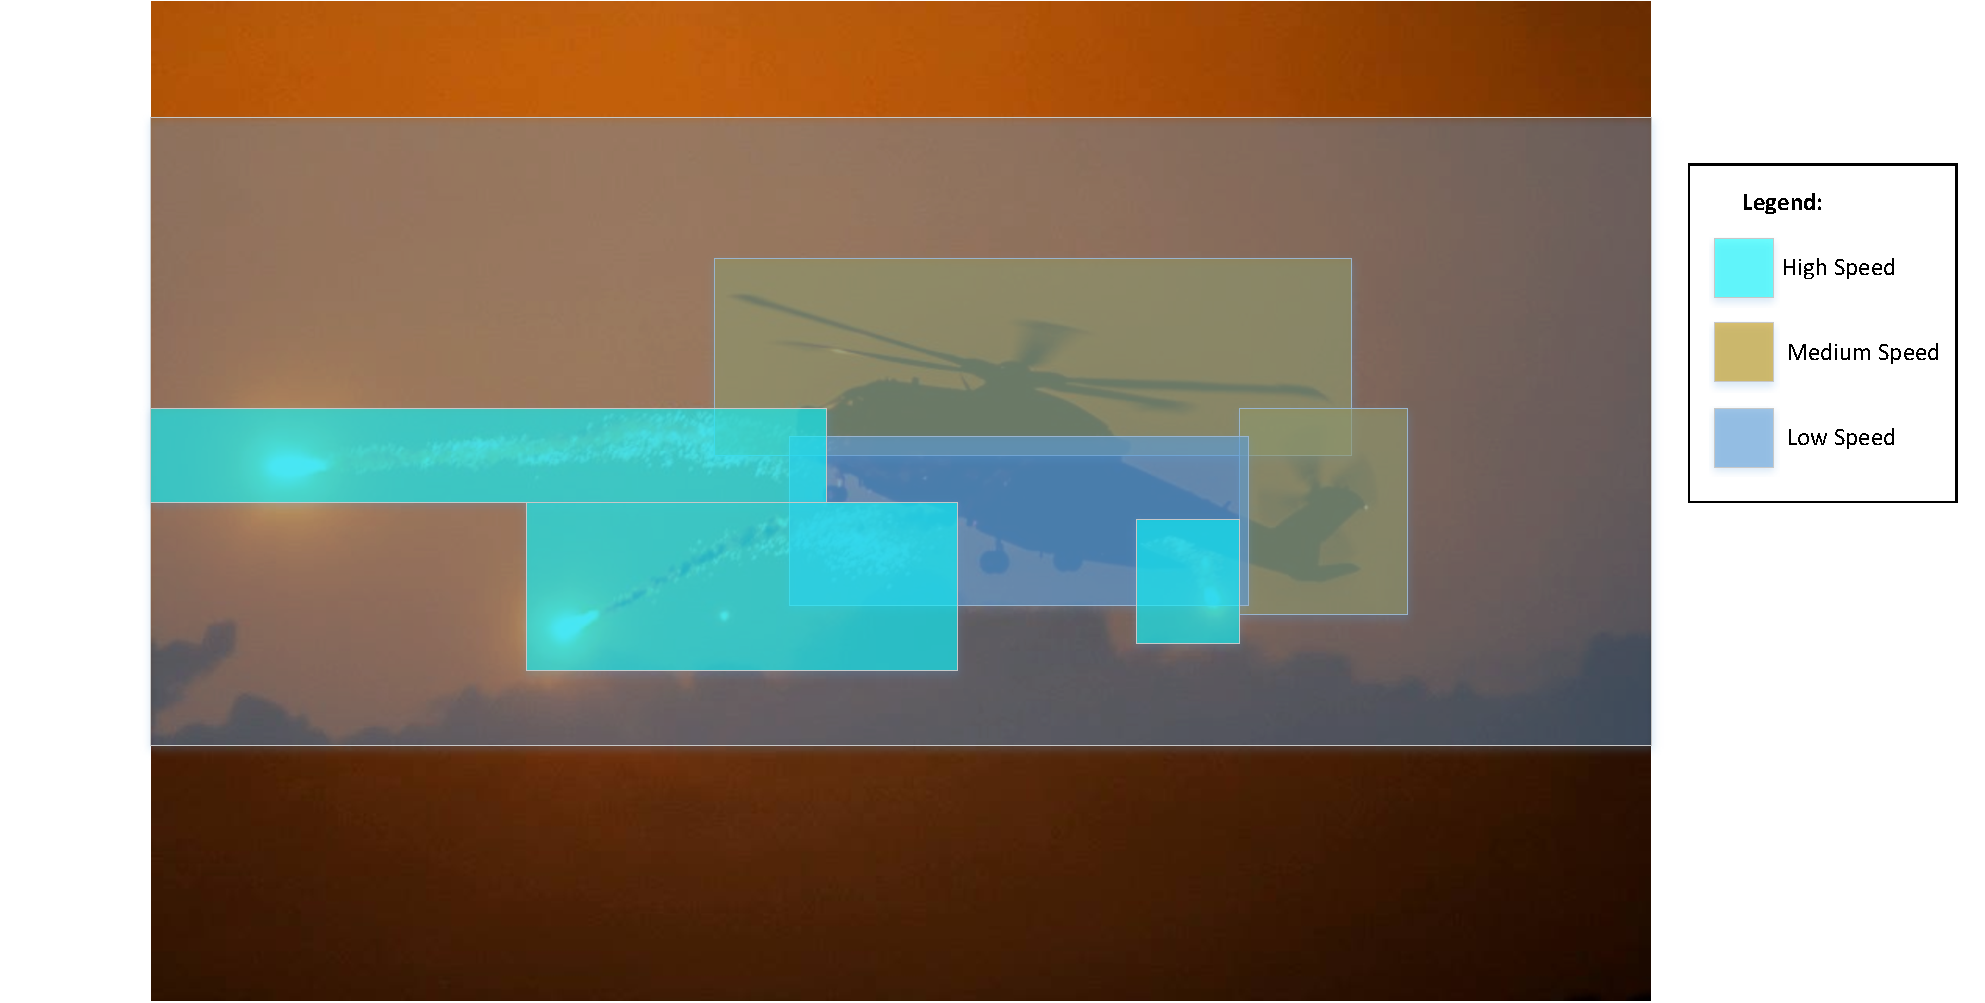
\includegraphics[width=1.0\textwidth]{fig/compositing_combined.pdf}
        \caption{Compositing Process Overlayed}
        \label{fig:compositing_overlayed}
    \end{figure}

    Consider the above scenario in the case of a single scene generator. In this case, the compositor receives data from a single source. As frame data is received, a differencing algorithm can be employed to determine how to segment the overall frame for optimal data transfer based off the rate of change for individual portions of the frame relative to the prior frame. Portions that rapidly change are sent more often than portions that change slowly in order to maximize bandwidth for high-speed display. This consequently also has the effect of improving the performance of the analog chain by allowing for devices to reserve more time to drive rapidly changing portions of a display over slowly changing portions. This is discussed in more detail shortly.

    In order to demonstrate how a differencing algorithm might be employed consider Figure~\ref{fig:intensity_map} which shows a series of composited frames with segmented regions that could be sent as individual PDP draw region packets to an array. Each region is a representation of the average intensity of all pixels contained within that region. Darker regions indicate higher intensity and lighter regions lower intensity. During the compositing process of each frame, the average intensity of light output for each segment could be computed. The outlined segments for a given frame indicate a large change in intensity from the previous frame. The compositor could then assign a weight to indicate which regions have a large absolute change in intensity from frame to frame. This information could then be utilized for deciding which segments of an image to send at high-speed operation or low speed operation. Segments with larger changes in intensity would be higher priority than segments with lower changes. The PDP could be utilized to send these regions at a much higher frame rate than the more slowly changing segments to reflect the fast changes in intensity. In practice, an implementation would likely utilize a rolling weighted score where regions with higher weighted scores would be sent more frequently than regions with lower scores; with the remaining bandwidth devoted to lower regions. Regions that could not be updated in a given frame would then have their priority increased for the next frame.

    \begin{figure}
        \centering
        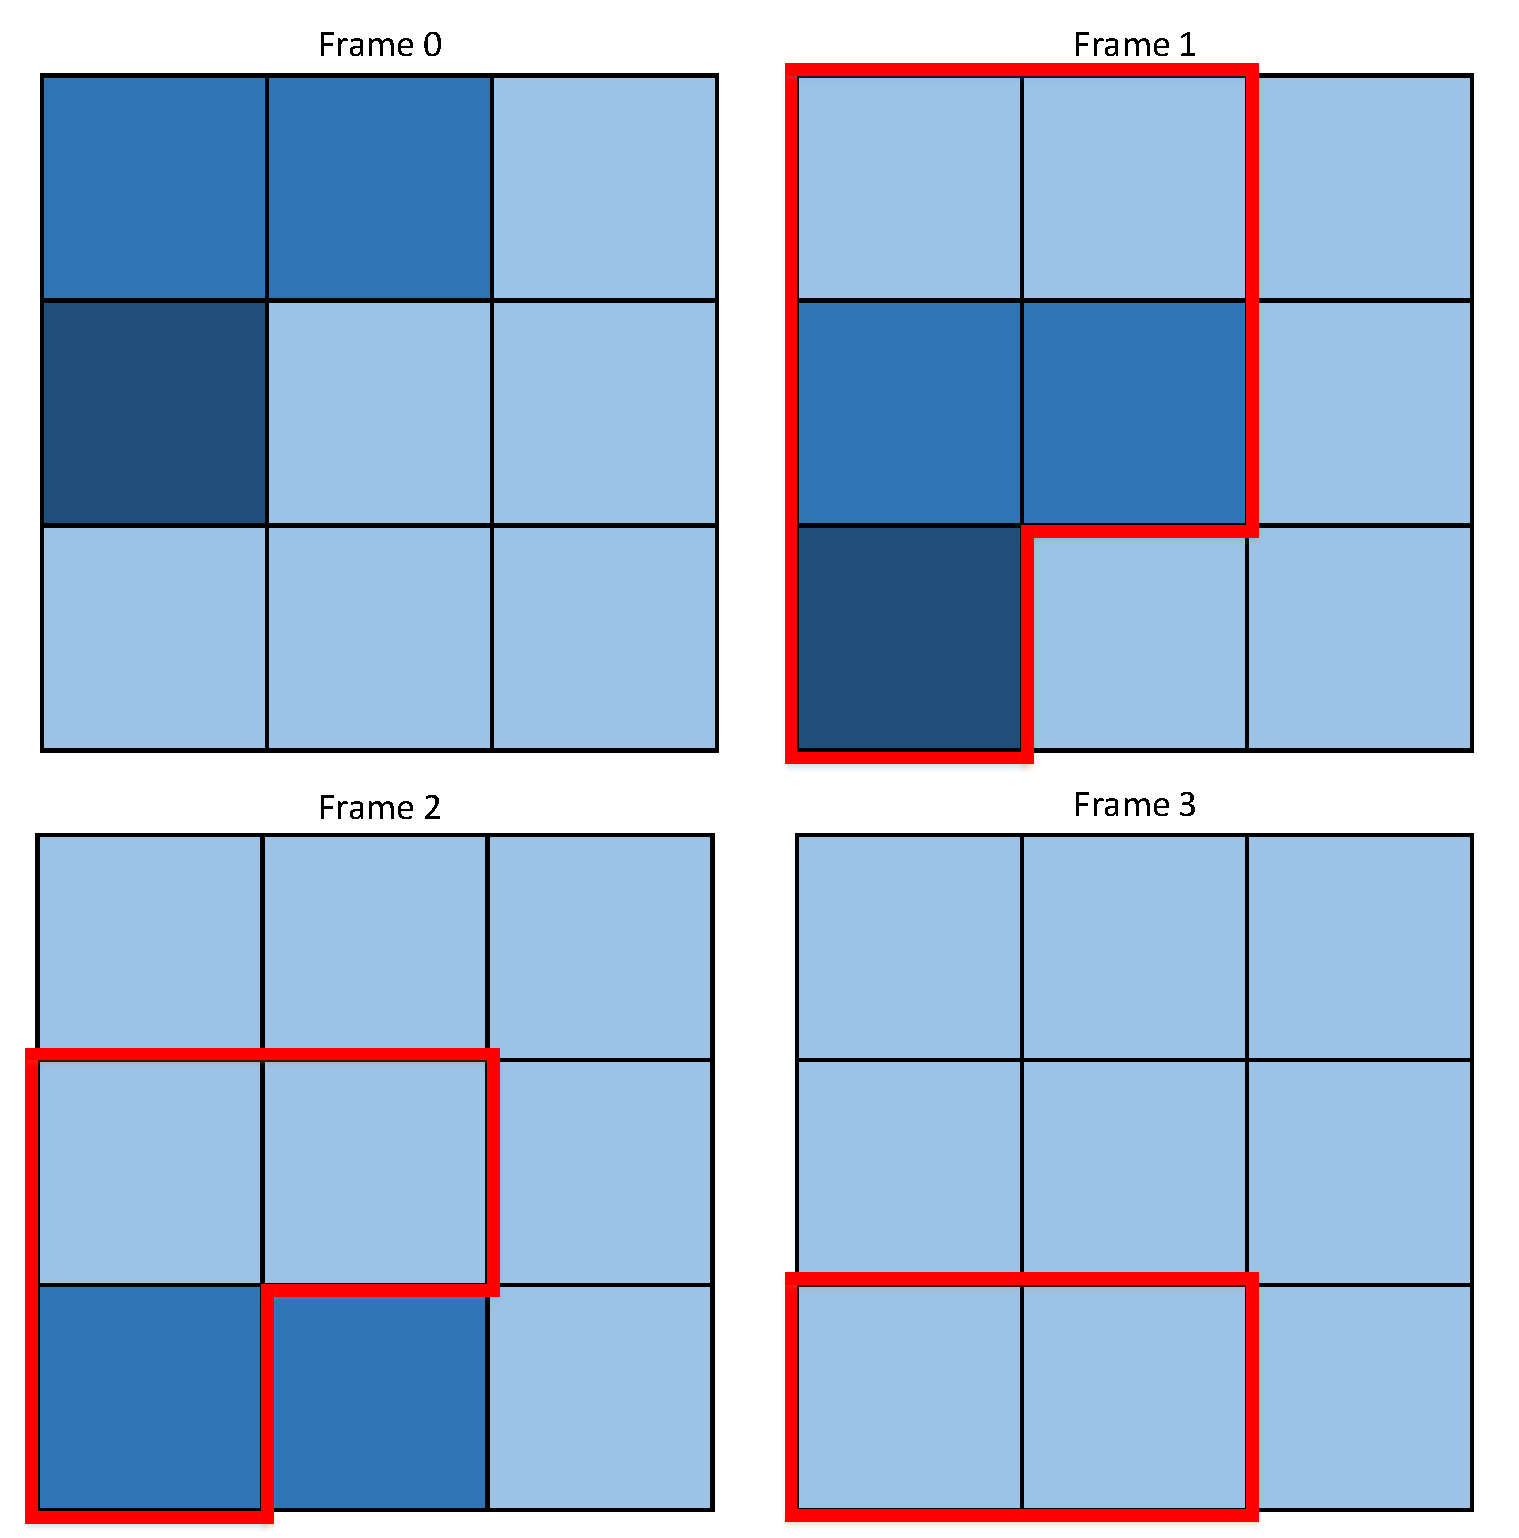
\includegraphics[width=0.85\textwidth]{fig/frames.pdf}
        \caption{Average Intensity Map of PDP Regions for Composited Frames}
        \label{fig:intensity_map}
    \end{figure}

    In a real system, frames would likely be segmented more finely than in this example, allowing for small segments to be dynamically transmitted, as necessary. This would then give the ability for fast changing data to update at rates far greater than a static fixed frame rate display would be capable of doing under the same hardware constraints. An added benefit is that by prioritizing segments, and decreasing the rates of slowly changing segments, more analog bandwidth can be utilized for drawing the high-speed portions of a display since the close support electronics no longer need to devote DAC and amplifier resources toward drawing low speed regions as often. Ultimately this would result in improved image fidelity by giving additional settling time to rapidly changing regions of an array. Though only touched upon in passing in Chapter~\ref{sec:array_Interleaved_write_process}, analog performance is of primary concern in IRSPs because a higher performance analog chain results in more consistent thermal output and an overall more thermally accurate image. Low analog performance can result in the same intensity data having different results over multiple captured frames due to DACs, amplifiers, and emitters not having the time to completely settle in high-speed operation.

    Now that all of the protocol level and abstract architectural details of the PDP have been discussed, the following chapter moves toward a discussion of an implementation of PDP on real hardware.
